\chapter{Metode Penelitian}

\section{Campus-Based LoRaWAN Architecture with Basic Station Gateway}
\label{subsec:campus_lorawan_architecture}

\begin{figure}[htbp]
    \centering
    % Replace with your actual image file (e.g., exported as PNG or PDF from draw.io)
    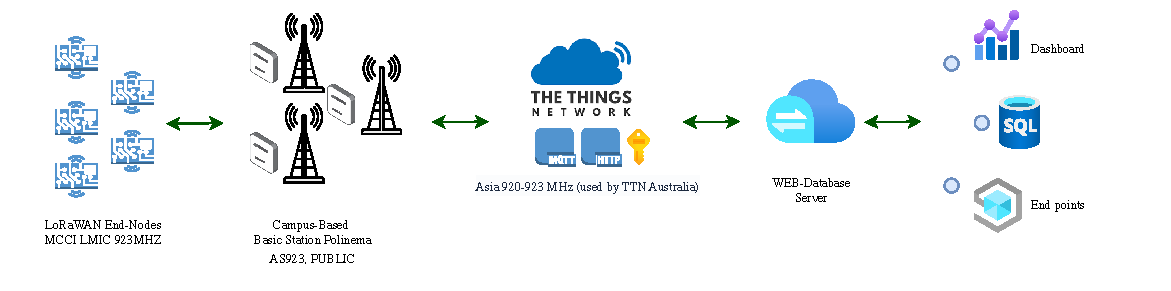
\includegraphics[width=0.95\textwidth]{../figures/cb-iot-arch.drawio.pdf}
    \caption{Campus-based LoRaWAN architecture using Basic Station gateway compliant with AS923 (Indonesia).}
    \label{fig:campuslorawanarch}
\end{figure}

Figure~\ref{fig:campuslorawanarch} illustrates the proposed campus-scale LoRaWAN architecture deployed at Polinema, utilizing the Basic Station gateway model compliant with Indonesian regulatory requirements. The system integrates end-devices, a LoRaWAN gateway, cloud infrastructure, and application endpoints into a cohesive IoT test bed. The components and data flow are described as follows:

\begin{enumerate}
    \item \textbf{LoRaWAN End-Nodes}
          \begin{enumerate}
              \item Located on the left side of the diagram, these represent sensor or actuator devices deployed across the campus (e.g., environmental monitors, smart meters).
              \item Each end-node is implemented using the MCCI LMIC stack configured for the \texttt{AS923} frequency plan (920–923 MHz), in accordance with Permenkominfo No. 21/2019.
              \item Devices transmit uplink messages using LoRa modulation and adhere to the 10\% duty cycle and 14 dBm EIRP power limit mandated for Indonesia.
          \end{enumerate}

    \item \textbf{Basic Station Gateway (Campus-Based)}
          \begin{enumerate}
              \item Positioned at the center-left, the gateway is labeled \textit{Campus-Based Basic Station Polinema} and operates in the \texttt{AS923 (PUBLIC)} mode.
              \item The gateway hardware (e.g., SenseCAP M1 or equivalent) runs the Basic Station software stack, enabling secure communication with The Things Network (TTN) via WebSocket over TLS.
              \item It receives LoRa frames from multiple end-nodes simultaneously across different spreading factors and channels within the 920–923 MHz band.
              \item The gateway forwards all received packets to the LoRaWAN Network Server (LNS) in the cloud using the LNS protocol, while also receiving downlink commands via the same secure channel.
          \end{enumerate}

    \item \textbf{Cloud Infrastructure (The Things Network)}
          \begin{enumerate}
              \item Represented by the central cloud icon, this layer corresponds to TTN’s \texttt{au1} or \texttt{eu1} cluster (configured as \texttt{AS923} for compatibility with Indonesian devices).
              \item The LNS performs frame validation, deduplication, and routing of application data to the appropriate integration endpoints.
              \item The gateway authenticates with TTN using its unique Gateway EUI and an API key, ensuring secure and authorized traffic exchange.
          \end{enumerate}

    \item \textbf{Application and Data Endpoints}
          \begin{enumerate}
              \item On the right side, three primary endpoints are shown:
                    \begin{enumerate}
                        \item \textit{Dashboard}: A web-based monitoring interface (e.g., Grafana, TTN Console) for real-time visualization of sensor data.
                        \item \textit{Time Series Data Sets}: A database or time-series storage system (e.g., InfluxDB, Azure Time Series Insights) for historical data logging and analytics.
                        \item \textit{Web-Database Server}: A custom application server hosting business logic, user management, and RESTful APIs for campus services (e.g., smart lighting, occupancy tracking).
                    \end{enumerate}
              \item Data flows from TTN to these endpoints via HTTP/MQTT integrations, as indicated by the protocol icons (HTTP, MQTT, and policy/access symbols) above the cloud layer.
          \end{enumerate}

    \item \textbf{Data Flow and Protocols}
          \begin{enumerate}
              \item Bidirectional arrows between components indicate full-duplex communication:
                    \begin{enumerate}
                        \item End-nodes $\leftrightarrow$ Gateway: LoRa RF communication (920–923 MHz, AS923).
                        \item Gateway $\leftrightarrow$ TTN: Secure WebSocket (port 8887) using Basic Station LNS protocol.
                        \item TTN $\leftrightarrow$ Endpoints: Standard internet protocols (HTTP/HTTPS, MQTT over TLS).
                    \end{enumerate}
              \item All cloud-to-application links are encrypted and authenticated, ensuring end-to-end security from sensor to dashboard.
          \end{enumerate}
\end{enumerate}

This architecture enables scalable, secure, and regulatory-compliant IoT deployment across the Polinema campus. By leveraging Basic Station and TTN, the system supports remote gateway management, over-the-air updates, and seamless integration with existing campus IT infrastructure—making it suitable for both research and operational use cases.



\section{Configuring Gateway: Basic Station}
\label{sec:configuring_gateway_basic_station}

This section provides a step-by-step guide to configuring a LoRaWAN gateway using the Basic Station software stack on The Things Network (TTN). The instructions are tailored for the Seeed Studio SenseCAP M1 gateway, which natively supports Basic Station and offers a user-friendly WebUI for initial setup.

\subsection{Setting-up Basic Station on TTN}
\label{subsec:basic_station_ttn_setup}

To integrate a Basic Station-compatible gateway (such as the SenseCAP M1) with The Things Network (TTN), the following steps must be performed. These steps assume the gateway has internet connectivity and has been powered on.

\begin{enumerate}
    \item \textbf{Create a Gateway Entry in The Things Network Console}
          \begin{enumerate}
              \item Log in to your account at \url{https://console.cloud.thethings.network/}.
              \item Navigate to the desired application or create a new one if necessary.
              \item In the left-hand menu, click on \textit{Gateways} and then select \textit{+ Add gateway}.
              \item Fill in the required fields:
                    \begin{enumerate}
                        \item \textit{Gateway ID}: Enter a unique, lowercase identifier (e.g., \texttt{univ-campus-gw-01}). This ID must be globally unique across TTN.
                        \item \textit{Gateway EUI}: Enter the 64-bit Gateway EUI (typically printed on the device label or found in the WebUI under device information). It must be entered in hexadecimal format without colons or dashes (e.g., \texttt{ABCDEF1234567890}).
                        \item \textit{Gateway Server Address}: Set to \texttt{eu1.cloud.thethings.network} (or the appropriate cluster region, e.g., \texttt{nam1}, \texttt{au1}, etc.).
                        \item \textit{Frequency Plan}: Select the correct regional plan. For Indonesia, choose \texttt{AS923} (specifically \texttt{AS923 - Group 1} or as defined by local regulations).
                        \item Leave other fields at their default values unless advanced configuration is required.
                    \end{enumerate}
              \item Click \textit{Create gateway}.
          \end{enumerate}

    \item \textbf{Obtain Gateway Authentication Credentials}
          \begin{enumerate}
              \item After creating the gateway, navigate to the gateway’s overview page in the TTN Console.
              \item Go to the \textit{General Settings} tab.
              \item Scroll down to the \textit{Gateway Authentication} section.
              \item Click \textit{Generate API key}.
              \item In the pop-up window:
                    \begin{enumerate}
                        \item Provide a name for the key (e.g., \texttt{basic-station-key}).
                        \item Under \textit{Rights}, ensure at least the following permissions are selected:
                              \begin{enumerate}
                                  \item \texttt{View gateway information}
                                  \item \texttt{Link as Gateway to a Gateway Server for traffic exchange}
                              \end{enumerate}
                        \item Click \textit{Create API key}.
                    \end{enumerate}
              \item Copy the generated API key immediately—it will not be shown again.
          \end{enumerate}

    \item \textbf{Configure the Gateway to Use TTN as LNS}
          \begin{enumerate}
              \item The SenseCAP M1 uses Basic Station, which requires two server endpoints:
                    \begin{enumerate}
                        \item \textit{LNS (LoRa Network Server)}: For real-time packet forwarding (e.g., \texttt{wss://[cluster].cloud.thethings.network:8887}).
                        \item \textit{CUPS (Configuration and Update Server)}: For secure provisioning and updates (e.g., \texttt{https://[cluster].cloud.thethings.network:443}).
                    \end{enumerate}
              \item These endpoints are typically configured automatically via the WebUI when TTN is selected as the network provider (see next subsection).
              \item The Gateway EUI and API key obtained above are used by the gateway to authenticate with TTN’s LNS and CUPS services.
          \end{enumerate}
\end{enumerate}

\subsection{Configuring Basic Station SenseCAP M1: WEBUI}
\label{subsec:sensecap_m1_webui}

The SenseCAP M1 provides a built-in web-based user interface (WebUI) accessible over Wi-Fi or Ethernet. The following steps detail the configuration process through this interface.

\begin{enumerate}
    \item \textbf{Access the WebUI}
          \begin{enumerate}
              \item Power on the SenseCAP M1 gateway.
              \item Connect your computer or mobile device to the gateway’s default Wi-Fi hotspot (SSID typically starts with \texttt{SenseCAP\_M1\_XXXX}).
              \item Open a web browser and navigate to \url{http://192.168.100.1}.
              \item Log in using the default credentials (usually username: \texttt{admin}, password: printed on the device label or set during first boot).
          \end{enumerate}

    \item \textbf{Connect to Local Network}
          \begin{enumerate}
              \item In the WebUI, go to \textit{Network Settings}.
              \item Configure internet connectivity:
                    \begin{enumerate}
                        \item For Wi-Fi: Select your campus or lab Wi-Fi network and enter the password.
                        \item For Ethernet: Ensure a cable is connected; DHCP is enabled by default.
                    \end{enumerate}
              \item Save settings and wait for the gateway to obtain an IP address on the local network.
              \item Note the new local IP address (e.g., \texttt{192.168.1.50}) to access the WebUI from the local network.
          \end{enumerate}

    \item \textbf{Select Network Provider}
          \begin{enumerate}
              \item Navigate to \textit{LoRaWAN Settings} or \textit{Network Provider}.
              \item Choose \textit{The Things Network (TTN)} from the list of available providers.
              \item The WebUI will automatically populate the following fields:
                    \begin{enumerate}
                        \item LNS Server: \texttt{wss://[region].cloud.thethings.network:8887}
                        \item CUPS Server: \texttt{https://[region].cloud.thethings.network:443}
                    \end{enumerate}
              \item If your region is not auto-detected, manually select the correct TTN cluster (e.g., \texttt{eu1} for Europe, \texttt{nam1} for North America). For Indonesia, \texttt{au1} or \texttt{eu1} may be used depending on latency and policy.
          \end{enumerate}

    \item \textbf{Enter Gateway Credentials}
          \begin{enumerate}
              \item In the same \textit{LoRaWAN Settings} section, enter the following:
                    \begin{enumerate}
                        \item \textit{Gateway EUI}: The 16-character hexadecimal EUI registered in TTN (e.g., \texttt{ABCDEF1234567890}).
                        \item \textit{API Key}: Paste the API key generated in Subsection~\ref{subsec:basic_station_ttn_setup}.
                    \end{enumerate}
              \item Ensure the \textit{Frequency Plan} is set to \texttt{AS923} to comply with Indonesian regulations (Permenkominfo No. 21/2019).
              \item Optionally, adjust the \textit{Transmission Power} and \textit{Duty Cycle} settings to respect the 14 dBm EIRP limit and 10\% duty cycle requirement for the 920–923 MHz band.
          \end{enumerate}

    \item \textbf{Apply and Reboot}
          \begin{enumerate}
              \item Click \textit{Save} or \textit{Apply Configuration}.
              \item The gateway will restart and initiate a secure WebSocket connection to TTN’s LNS using TLS.
              \item Monitor the WebUI status page for connection indicators (e.g., “Connected to LNS”).
          \end{enumerate}

    \item \textbf{Verify Operation in TTN Console}
          \begin{enumerate}
              \item Return to the TTN Console gateway page.
              \item Check the \textit{Live Data} tab to confirm uplink messages are being received.
              \item Verify that the gateway status shows as \textit{Connected}.
              \item If no data appears, check:
                    \begin{enumerate}
                        \item Internet connectivity of the gateway,
                        \item Correctness of Gateway EUI and API key,
                        \item Regional frequency plan alignment (AS923 for Indonesia),
                        \item Firewall or proxy settings that may block WebSocket (port 8887) or HTTPS (port 443) traffic.
                    \end{enumerate}
          \end{enumerate}
\end{enumerate}


\section{End-Nodes Using Lilygo T3S3}
\label{sec:end_nodes_lilygo_t3s3}
The end-nodes for this campus-based LoRaWAN architecture are implemented using the Lilygo T3S3 development board, which features the ESP32 microcontroller and an integrated SX1276 LoRa transceiver. The following outlines the configuration and programming steps to set up the Lilygo T3S3 as LoRaWAN end-nodes compliant with the AS923 frequency plan.
\subsection{Hardware Setup}
\begin{enumerate}
    \item \textbf{Lilygo T3S3 Board}
          \begin{enumerate}
              \item Ensure you have the Lilygo T3S3 board with the SX1276 LoRa module.
              \item Connect the board to your computer via USB for programming and power.
          \end{enumerate}
    \item \textbf{Antenna Connection}
          \begin{enumerate}
              \item Attach a suitable antenna for the 920–923 MHz frequency range to the LoRa module to ensure optimal signal transmission and reception.
          \end{enumerate}
\end{enumerate}
\subsection{Software Setup}
\begin{enumerate}
    \item \textbf{Arduino IDE Configuration}
          \begin{enumerate}
              \item Install the Arduino IDE if not already installed.
              \item Add the ESP32 board support by including the following URL in the Additional Board Manager URLs: \url{https://dl.espressif.com/dl/package_esp32_index.json}.
              \item Install the ESP32 board package via the Board Manager.
              \item Select the Lilygo T3S3 board from the Tools > Board menu.
          \end{enumerate}
    \item \textbf{Library Installation}
          \begin{enumerate}
              \item Install the MCCI LoRaWAN LMIC library via the Library Manager (Sketch > Include Library > Manage Libraries).
              \item Ensure the library version supports the AS923 frequency plan.
          \end{enumerate}
\end{enumerate}
\subsection{Programming the End-Nodes}
\begin{enumerate}
    \item \textbf{LoRaWAN Configuration}
          \begin{enumerate}
              \item Configure the LMIC library for the AS923 frequency plan by defining the appropriate parameters in your sketch.
              \item Set the device EUI, application EUI, and application key as provided by TTN for your end-node.
          \end{enumerate}
    \item \textbf{Uplink Message Implementation}
          \begin{enumerate}
              \item Implement code to read sensor data (e.g., temperature, humidity) and format it into a payload suitable for LoRaWAN transmission.
              \item Use the LMIC library functions to send uplink messages at defined intervals, adhering to duty cycle regulations.
          \end{enumerate}
    \item \textbf{Testing and Deployment}
          \begin{enumerate}
              \item Upload the sketch to the Lilygo T3S3 board.
              \item Monitor the TTN Console to verify that uplink messages are being received correctly.
              \item Deploy the end-nodes across the campus as needed, ensuring they are within range of the gateway.
          \end{enumerate}
\end{enumerate}

\subsection{LoRaWAN TTN End-Device Registration}
To register the Lilygo T3S3 end-nodes on The Things Network (TTN), follow these steps:
\begin{enumerate}
    \item Log in to your TTN Console account.
    \item Navigate to the application where you want to register the end-device.
    \item Click on \textit{End devices} and then select \textit{+ Add end device}.
    \item Fill in the required fields:
          \begin{enumerate}
              \item \textit{End device ID}: A unique identifier for the end-device (e.g., \texttt{lilygo-t3s3-node-01}).
              \item \textit{Device EUI}: The 64-bit unique identifier for the device, which can be generated or obtained from the board.
              \item \textit{Application EUI}: The 64-bit identifier for the application, provided by TTN.
              \item \textit{App Key}: A 128-bit key used for encryption, also provided by TTN.
              \item \textit{Frequency Plan}: Select \texttt{AS923} to comply with Indonesian regulations.
              \item Leave other fields at their default values unless specific configurations are needed.
              \item Click \textit{Create end device}.
              \item Repeat the process for each Lilygo T3S3 end-node you wish to register.
              \item After registration, monitor the \textit{Live Data} tab for each end-device to verify successful uplink message reception.
              \item Ensure that the end-nodes are configured to use OTAA (Over-The-Air Activation) for secure network joining.
              \item Deploy the end-nodes in their intended locations and ensure they are within range of the gateway for optimal performance.
          \end{enumerate}
\end{enumerate}

Table~\ref{tab:TTN_frequency_plans} summarizes the frequency plans available on TTN, highlighting the AS923 plan used in this architecture.
\begin{table}[htbp]
    \centering
    \caption{TTN Frequency Plans Summary}
    \label{tab:TTN_frequency_plans}
    \begin{tabular}{|c|c|c|c|}
        \hline
        \textbf{Frequency Plan} & \textbf{Region}          & \textbf{Uplink Frequencies (MHz)} & \textbf{Downlink Frequencies (MHz)} \\ \hline
        AS923                   & Asia-Pacific (Indonesia) & 920-923                           & 920-923                             \\ \hline
        EU868                   & Europe                   & 863-870                           & 863-870                             \\ \hline
        US915                   & North America            & 902-928                           & 923-927                             \\ \hline
        AU915                   & Australia                & 915-928                           & 923-928                             \\ \hline
        CN470                   & China                    & 470-510                           & 470-510                             \\ \hline
    \end{tabular}
\end{table}

\subsection{LoRaWAN specifications and Regional Parameters}
The Lilygo T3S3 end-nodes are configured to operate under the LoRaWAN specifications defined for the AS923 frequency plan, which is compliant with Indonesian regulations as per Permenkominfo No. 21/2019. Key specifications include:
\begin{itemize}
    \item \textbf{Frequency Range}: 920–923 MHz for both uplink and downlink communications.
    \item \textbf{Maximum EIRP}: 14 dBm, adhering to local regulatory limits.
    \item \textbf{Duty Cycle}: 10\% maximum duty cycle for transmissions to minimize interference.
    \item \textbf{Spreading Factors}: Configurable from SF7 to SF12, allowing for trade-offs between data rate and range.
    \item \textbf{Channel Plan}: Multiple channels are defined within the AS923 plan to support simultaneous transmissions from multiple end-nodes.
    \item \textbf{Data Rates}: Ranging from DR0 (SF12, 250 bps) to DR5 (SF7, 5470 bps), enabling flexible communication based on application requirements.
\end{itemize}

Table~\ref{tab:lorawan_specifications} shows LoRaWAN versions and specifications available in TTN.
\begin{table}[htbp]
    \centering
    \caption{LoRaWAN Versions and Specifications in TTN}
    \label{tab:lorawan_specifications}
    \begin{tabular}{|c|c|c|c|}
        \hline
        \textbf{LoRaWAN Version} & \textbf{Max Payload Size (bytes)} & \textbf{Max Data Rate (bps)} & \textbf{Spreading Factors} \\ \hline
        1.0.0                    & 51                                & 5470                         & SF7 to SF12                \\ \hline
        1.0.1                    & 51                                & 5470                         & SF7 to SF12                \\ \hline
        1.0.2                    & 222                               & 5470                         & SF7 to SF12                \\ \hline
        1.0.3                    & 222                               & 5470                         & SF7 to SF12                \\ \hline
        1.1                      & 242                               & 5470                         & SF7 to SF12                \\ \hline
    \end{tabular}
\end{table}

Regional parameter is defined in Table~\ref{tab:regional_parameters} shows regional parameters versions available on TTN and its description.
RP001 Regional Parameters 1.0.3 revision A is used for AS923 frequency plan.
Describes all option avaliable for regional pa




\section{Tahapan Penelitian}
Langkah-langkah yang harus dilakukan (lihat Gambar~\ref{fig:tahapan_penelitian}) untuk menyelesaikan penelitian ini dengan baik yang juga memungkinkan untuk menghasilkan prototipe yang dapat digunakan pada laboratorium sistem kontrol, serta tulisan yang dapat dipresentasikan pada seminar internasional terindeks IEEE, dan dokumen feasibility study, implementation arrangement, KI, untuk tujuan komersialisasi prototipe adalah sebagai berikut:

\begin{enumerate}
    \item Penelitian dan Studi Literatur yang Mendalam.  Langkah awal yang krusial adalah melakukan penelitian dan studi literatur yang menyeluruh terkait dengan Model Predictive Control (MPC), sistem kontrol, serta pengembangan prototipe perangkat keras. Tersedianya informasi yang tepat dan pemahaman yang kuat merupakan kunci utama untuk memulai penelitian ini dengan baik. Indikator Keberhasilan: Identifikasi jurnal terkemuka, buku, dan sumber daya tepercaya tentang Model Predictive Control (MPC) dan sistem kontrol. Membangun pemahaman yang kuat tentang konsep MPC, sejarah, dan penerapannya.
    \item Identifikasi Spesifikasi Prototipe. Selanjutnya adalah mengidentifikasi spesifikasi dan persyaratan yang diperlukan untuk mengembangkan prototipe yang dapat digunakan pada laboratorium sistem kontrol. Ini meliputi desain perangkat keras yang cocok, pilihan perangkat lunak yang tepat, serta integrasi komponen yang diperlukan sesuai kebutuhan. Indikator Keberhasilan: Dokumen spesifikasi yang jelas dan terinci yang mencakup persyaratan perangkat keras, perangkat lunak, output yang diharapkan, dan kriteria evaluasi prototipe.
    \item Desain Perangkat Keras dan Perangkat Lunak. Setelah spesifikasi prototipe teridentifikasi, langkah selanjutnya adalah merancang perangkat keras dan perangkat lunak yang sesuai dengan persyaratan yang ada. Ini mencakup pemilihan komponen, perancangan sirkuit, dan implementasi perangkat lunak untuk kontrol dan interaksi sistem. Indikator Keberhasilan: Penyelesaian desain perangkat keras yang dilengkapi dengan skematik dan layout PCB, serta pengembangan perangkat lunak dengan beroperasinya fungsi kontrol sesuai spesifikasi.
    \item Pengujian dan Evaluasi. Prototipe yang dikembangkan harus diuji secara ekstensif, baik untuk memastikan kinerja yang diharapkan maupun untuk memverifikasi bahwa prototipe tersebut sesuai dengan spesifikasi yang telah ditetapkan. Indikator Keberhasilan: Pengujian prototipe yang menghasilkan data kuantitatif dan kualitatif untuk mengevaluasi kinerja prototipe sesuai dengan spesifikasi yang ditetapkan.
    \item Penulisan Paper Ilmiah dan KI. Selama proses pengembangan prototipe, penting untuk secara bersamaan mulai menulis paper ilmiah yang mendokumentasikan konsep, perancangan, pengujian, dan hasil dari penelitian ini. Paper ini harus dirancang sejak awal agar memenuhi standar dan persyaratan yang diperlukan untuk mempresentasikan penelitian dalam konferensi internasional terindeks seperti IEEE. Pada tahap ini, dituliskan juga dokumen KI untuk program komputer. Indikator Keberhasilan: Penyusunan sepenuhnya paper ilmiah dengan latar belakang yang kuat, tujuan penelitian yang jelas, metodologi yang tepat, hasil yang signifikan, dan kesimpulan yang terdefinisi dengan baik, serta sertifikat KI.
    \item Analisis Kelayakan Bisnis. Sambil mengembangkan prototipe, langkah selanjutnya adalah melakukan analisis kelayakan bisnis atau feasibility study. Ini mencakup analisis pasar, potensi komersialisasi, dan strategi pemasaran yang dapat diterapkan jika prototipe berhasil dikembangkan. Indikator Keberhasilan: Dokumen analisis kelayakan bisnis yang mencakup analisis risiko, evaluasi pasar yang komprehensif, strategi pemasaran yang efektif, dan proyeksi pendapatan.
    \item Penulisan Dokumen Feasibility Study dan Implementation Arrangement. Berdasarkan hasil analisis kelayakan bisnis, selanjutnya diperlukan pengembangan dokumen feasibility study yang komprehensif, mencakup analisis pasar, rencana pemasaran, perkiraan pendapatan, dan informasi terkait komersialisasi prototipe. Indikator Keberhasilan: Diselesaikannya dokumen feasibility study yang menyediakan gambaran yang jelas tentang potensi komersialisasi, rencana pemasaran, target pasar, dan strategi untuk memasarkan prototipe.
    \item Presentasi pada Seminar Internasional. Setelah paper ilmiah selesai, adalah mendaftar untuk mengajukan presentasi pada konferensi atau seminar internasional terindeks seperti IEEE. Proses penerimaan untuk konferensi ini sering kali memerlukan penyerahan paper yang ketat dan sesuai kriteria. Indikator Keberhasilan: Penyerahan paper ilmiah yang lulus seleksi peer-review dan diterima oleh konferensi, serta presentasi yang mengesankan dan informatif pada seminar internasional yang terindeks.
    \item Pelaporan Akhir Penelitian. Langkah terakhir adalah pelaporan penelitian: Indikator tersedianya dokumen yang diperlukan untuk pelaporan penelitian.
\end{enumerate}

\section{Uraian Tugas Ketua, Anggota Peneliti dan Mitra}
Pembagian dan uraian tugas ketua peneliti dan anggota peneliti serta mitra adalah sebagai berikut:
\begin{enumerate}
    \item Ketua:
          \begin{enumerate}
              \item Merencanakan Usulan (Proposal, Administrasi, RAB, Monev, dan Hasil), perumusan sistem kontrol
              \item Mendisain, mengimplementasikan dan menguji algoritma sistem kontrol
              \item Mengintegrasikan sistem dan sub-sub sistem dalam diagram kontrol
              \item Memprogram algoritma MPC
              \item Menyusun dan presentasi artikel publikasi pada seminar
              \item Menyusun dan melaporkan luaran dan laporan untuk monev dan laporan akhir
              \item Menyusun feasibility study, implementation arrangement dan dokumen hak cipta
          \end{enumerate}
    \item Anggota 1:
          \begin{enumerate}
              \item Mendisain sistem travel cart-inverted pendulum
              \item Mendisain sistem belt-drive dan sistem gear
              \item Mendisain linear actuator
              \item Membantu analisa data
          \end{enumerate}
    \item Anggota 2:
          \begin{enumerate}
              \item Mendisain sistem elektronik power-supply
              \item Mendisain sistem elektronik komunikasi
              \item Mendisain sistem elektronik embedded sistem
              \item Membantu analisa data
          \end{enumerate}
    \item Anggota 3:
          \begin{enumerate}
              \item Menyusun algoritma pemrograman sistem komputasi matrix dan vector
              \item Menyusun algoritma pemrograman sistem komputasi integrator
              \item Menyusun algoritma pemrograman system optimasi
              \item Mendisain layout plotting respon sistem
          \end{enumerate}
    \item Mahasiswa:
          \begin{enumerate}
              \item Membantu realisasi sistem mekanik dengan peralatan-peralatan rapid-prototyping: 3D Printer, CNC, dll.
              \item Membantu realisasi disain sistem komputasi dan antarmuka dengan Bahasa pemrograman Python
              \item Membantu realisasi disain sistem elektronik dengan software rangkaian elektronik serta mesin pembuat PCB
          \end{enumerate}
    \item Mitra Industri
          \begin{enumerate}
              \item Membantu menyusun feasibility study dan dokumen implementation arrangement
              \item Memberikan spesifikasi-spesifikasi detil tentang produk sesuai dengan permintaan pasar dan kondisi produk-produk serupa yang di pasaran
              \item Membantu menentukan parameter-paremeter teknis CAD/CAM untuk disain prototipe
              \item Membantu merencanakan disain elektronik, komunikasi dan mekanik
              \item Memberikan dukungan dengan penyediaan sarana dan prasarana yang dimiliki mitra untuk dapat digunakan dalam proses rapid prototyping
          \end{enumerate}
\end{enumerate}




